\chapter{Private-Key Cryptography}
%\newcommand{\key}{\mathsf{k}}
% \newcommand{\gen}{\mathsf{Gen}}
\section{Private-Key Encryption}
The first primitive that we will study in private-key cryptography is that of private-key encryption.
When talking about private-key encryption, we will be working in a setting where two players, Alice and Bob, are attempting to communicate with each other.

Alice and Bob want to communicate with each other.
For simplicity, let's assume that only Alice wants to send a message to Bob.
The crucial property that they want is that no eavesdropper attempting to listen to the conversation should be able to decipher the contents of the message being sent.
\begin{comment}
\begin{center}
    \begin{tikzpicture}
        \draw;
    \end{tikzpicture}
\end{center}    
\end{comment}
% Figure A goes here

To achieve this, the two employ the following communication protocol:
\begin{enumerate}
    \item A priori, Alice and Bob generate a key $k$ and distribute it in such a way that only the two of them know what $k$ is.
    \item Using $k$, Alice can encrypt her message $m$, to turn it into a ciphertext $c$, which she sends over to Bob. 
    \item Upon receiving $c$, Bob can decrypt its contents and recover $m$ by using $k$.
\end{enumerate}
This meta-scheme implies a couple of requirements.
First of all, we want Bob to indeed be able to recover $m$ when decrypting $c$ with $k$.
It is no use having a communication scheme where the message received is not the one sent. We will call this requirement \textit{correctness}.
The second requirement, which we have already mentioned, is \textit{confidentiality}.
To reiterate, \textit{confidentiality} means that no eavesdropper that manages to get a hold of $c$ should be able to learn anything about $c$ that they do not already know (assuming they have no knowledge of the key $k$).
In addition to these two fundamental requirements, we might also impose that our private-key encryption scheme guarantees \textit{integrity} and \textit{authenticity}.
By \textit{integrity}, we mean that Bob should be able to detect that the message $c$ has been tampered with prior to him receiving it.
By \textit{authenticity}, we mean that Bob should be able to verify that the message he received was indeed sent by Alice, and not some adversary interfering with the conversation.

Now that we have some intuitive understanding of what we are trying to achieve, let us attempt to ground it in mathematics.

\begin{definition}[Private-Key Encryption Scheme]
    A private-key encryption scheme $\Pi$ is a tuple $\Pi = (\gen, \enc, \dec)$, where $\gen, \enc$, and $\dec$ are algorithms such that:
    \begin{enumerate}
        \item $\gen(1^n) \rightarrow k$
        \item $\enc(k, m) \rightarrow c$
        \item $\dec(k, c) \rightarrow m'$
    \end{enumerate}
    
    where $n$ is a security parameter and $k, c, m, m' \in \{0, 1\}^*$
\end{definition}


%Alice might also want to be able to deal with attackers that can tamper with $c$.
%When Bob receives something, he wants to be able to verify that it indeed comes from Alice.

\begin{comment}
$$\Pi = (Gen, Enc, Dec)$$
$$Gen(1^n) \rightarrow k$$
$$Enc(k, m) \rightarrow c$$
$$Dec(k, c) \rightarrow m'$$
\end{comment}


% Besides correctness, we want our cryptosystem to be \textit{confidential}.

Now, we will formalize the requirements of our cryptosystem.
Our first requirement is correctness, which is defined below:

\begin{definition}[(Perfect) Correctness]
    We say that a private-key encryption scheme $\Pi = (\gen, \enc, \dec)$ is \emph{(perfectly) correct} if 
    $\forall n, k \in \gen(1^n), m \in \{0,1\}^{*}$,
    $$\Pr[\dec(k,\enc(k,m)) = m] = 1$$
\end{definition}
That is, if $c = \enc(k, m)$, then Bob is guaranteed to recover $m$ by running $\dec(k, c)$. Note that for a fixed-length encryption scheme, we require that $m \in \bit^{l(n)}$.

Next, we will formalize what we mean by \textit{confidentiality}.
We will often use the terms \textit{confidentiality} and \textit{security} interchangeably in the context of private-key encryption schemes.
Our first definition of confidentiality is called IND Security, stated below:

\begin{definition}[IND Security]
    $\forall m_0, \forall m_1$ s.t. $|m_0| = |m_1|= l(n)$ and $\forall$ nu-PPT $\ma$ we have
    $$|\Pr[\ma(1^n, \enc(k, m_0)) = 1 \; | \; k \leftarrow \gen(1^n)] - |\Pr[\ma(1^n, \enc(k, m_1)) = 1 \; | \; k \leftarrow \gen(1^n)]| = neg(n)$$ 
\end{definition}
Note that this is not a particularly good definition of security, in the sense that the attacker is very limited in what they are allowed to do.
Specifically, all that $\ma$ can do is take a look at the encryption of $m_0$ and $m_1$ and must decide which one is the plaintext.
We need a more usable and realistic definition of security.
For this reason, we will allow the attacker to have oracle access to the encryption function, $\enc(k, \cdot)$.
In other words, $\ma$ will be able to craft their own ciphertexts, which it can then use to break the security of the encryption scheme.
We shall dub this new definition of security \textit{Chosen Plaintext Attack Security}, or \textit{CPA Security} for short.

%Informally, this means that the ciphertext $c$ should hide everything about $m$ that Eve doesn't already know.

In defining \textit{CPA Security}, we will also introduce a new method for defining private-key encryption schemes: the game-style definition.
The rationale behind this change in style is that probabilistic definitions, while precise and rigorous, are rather cumbersome to work with, especially in the context of secure communication.
Therefore, we will adopt this new paradigm, which will make it easier to work with and reason about private-key encryption schemes.

\marginnote[-1.5in]{
\procedureblock[linenumbering]{$ \pcnotionstyle{Priv\pcmathhyphen{}}\indcpa_{\Pi}^{\adv}(\secpar)$}{
 b \getsr \bin \\
  \key  \getsr \gen ( \secparam ) \\
 ( \state ,m_0 ,m_1) \getsr \adv^{\enc ( \key ,\cdot )} ( \secparam) \\
 c \getsr \enc ( \key ,m_b ) \\
 b' \getsr \adv^{\enc ( \key ,\cdot )} ( \state , c ) \\
 \pcreturn b = b' \land |m_0| = |m_1| = l(n)
 }}

\begin{definition}[CPA Security]
    A private-key encryption scheme $\Pi = (\gen,\enc,\dec)$ is CPA-secure if $\forall$ nu-PPT $\ma$
    $$\advantage{\indcpa}{\Pi,\adv} = \Big| \Pr[\pcnotionstyle{Priv\pcmathhyphen{}}\indcpa_\Pi^\adv(\secpar) =1] -\frac12\Big|$$
    is a negligible function.
\end{definition}
Observe that in this new game-style definition, we have a concrete notion of the order in which each action is taken.
One important detail to note (and that is more evident in a game-style definition) is that in our \textit{CPA Security} definition,
the key $k$ is sampled \textit{before} $m_0$ and $m_1$ are fixed.
This is in contrast to \textit{IND Security}, in which the messages $m_0$ and $m_1$ are chosen before the key $k$ is sampled\footnote{This is an important detail because if $m_0$ and $m_1$ are chosen before $k$ is sampled, then giving oracle access to $\ma$ is not much help.}.

To further illustrate this point, consider the following scheme, which is secure in IND but insecure in CPA:
\begin{itemize}
    \item $\gen(\secparam):$
    \begin{enumerate}
        \item $k \leftarrow \gen(\secparam)$
        \item $x \getsr \{0, 1\}^n$
        \item $k' = (k, x)$
    \end{enumerate}
    \item $\enc'(k', m)L:$
    \begin{enumerate}
        \item if $m = x$, then output $x$
        \item else, output $\enc(k,m)||x$
    \end{enumerate}
\end{itemize}

%We formalize this property in our definition of \emph{Chosen Plaintext Attack Security}, or \textit{CPA Security} for short.
%In presenting this new definition, we will also introduce the notion of game-style definitions.
%The motivation behind this is that probabilistic definitions, such as the ones we have been working with thus far, are cumbersome and difficult to work with.
%Game-style definitions are easier to work with and give us better ideas of 

%Properties we want:
%\begin{itemize}
%    \item $c$ should hide everything about $m$ that Eve doesn't already know
%\end{itemize}

%There are many ways to formally define this notion
%Formally,

% To make this definition of security more robust, we allow $\ma$ to have oracle access\footnote{In other words, $\ma$ can create their own ciphertexts.} to $\enc(k, \cdot)$
% This definition is not good enough because we are fixing $m_0$ and $m_1$. * ASK ABOUT THIS.

\begin{comment}
\begin{definition}[$\pcnotionstyle{Priv\pcmathhyphen{}}\indcpa$] A private-key encryption scheme $\Pi = (\gen,\enc,\dec)$ is $\pcnotionstyle{Priv\pcmathhyphen{}}\indcpa$-secure if 
$$ \advantage{\indcpa}{\Pi,\adv} = \Large\mid \Pr[\pcnotionstyle{Priv\pcmathhyphen{}}\indcpa_\Pi^\adv(\secpar) =1] -\frac12\Large\mid$$
is a negligible function. 
\end{definition}    
The main difference is when the key $k$ is sampled.
In the first definition, $m_0$ and $m_1$ are fixed before $k$ is sampled,
whereas in the second definition, $k$ is sampled before $m_0$ and $m_1$ are fixed.
\end{comment}

% Transition from the probability-style definitions to game-style definitions.


The final security notion we will define is CCA (chosen-ciphertext attack) security.
Here, the attacker is allowed oracle access to both the encryption and the decryption functions.
Let $L$ be the working list of queries that $\ma$ has made to $Dec(k, \cdot)$.
Then $\pcnotionstyle{Priv\pcmathhyphen{}}\indcca_{\Pi}^{\adv}(\secpar)$ is defined as:
\marginnote[-1.5in]{
\procedureblock[linenumbering]{$ \pcnotionstyle{Priv\pcmathhyphen{}}\indcca_{\Pi}^{\adv}(\secpar)$}{
 b \getsr \bin \\
  \key  \getsr \gen ( \secparam ) \\
 ( \state ,m_0 ,m_1) \getsr \adv^{\enc ( \key ,\cdot ), \dec(k, \cdot)} ( \secparam) \\
 c \getsr \enc ( \key ,m_b ) \\
 b' \getsr \adv^{\enc ( \key ,\cdot ), \dec(k, \cdot)} ( \state , c ) \\
 \pcreturn b = b' \land |m_0| = |m_1| \land c \notin L
 }}

\begin{definition}[CCA Security]
    A private-key encryption scheme $\Pi = (\gen,\enc,\dec)$ is CCA-secure if $\forall$ nu-PPT $\ma$
    $$\advantage{\indcca}{\Pi,\adv} = \Big| \Pr[\pcnotionstyle{Pri\pcmathhyphen{}}\indcca_\Pi^\adv(\secpar) =1] -\frac12\Big|$$
    is a negligible function.
\end{definition}

$\Pi$ is a fixed-length encryption scheme for length $l(n)$ if $l(n)$ is polynomial in $n$ and $|m_0| = |m_1| = l(n)$.

\begin{theorem}
    If F is a PRF then the scheme $\Pi = (\gen, \enc, \dec)$ given below is a secure encryption scheme for length $n$.

    \begin{itemize}
        \item $\gen(\secparam)$:
        \begin{enumerate}
            \item output $k \getsr \{0, 1\}^n$
        \end{enumerate}
        \item $\enc(k, m)$:
        \begin{enumerate}
            \item $r \getsr \{0, 1\}^n$
            \item output $(r, F_k(r) \oplus m)$
        \end{enumerate}
        \item $\dec(k, c=(c_1, c_2))$:
        \begin{enumerate}
            \item output $c_2 \oplus F_k(c_1)$
        \end{enumerate}
    \end{itemize}
    
\end{theorem}

\proof
Assume there exists a nu-PPT $\ma$ that is able to break CPA security of $\Pi$.
Then we can construct a nu-PPT adversary $\mb$ that breaks the PRF $F$.
The strategy is outlined in the figure below:

\begin{center}
    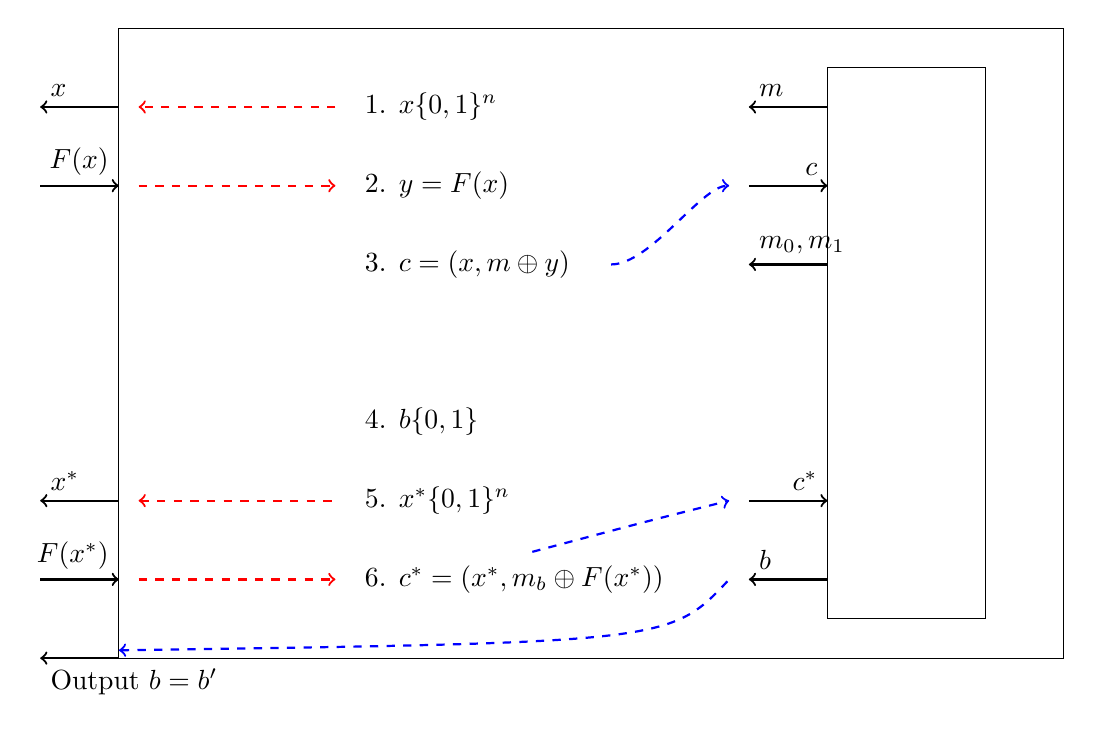
\begin{tikzpicture}
        % Adversary B rectangle
        \draw (0,8) node[anchor=north west]{$\mb$};
        \draw (0, 0) rectangle (12, 8);
        \draw[thick, ->] (0,7)--(-1,7) node[anchor=south west] {$x$};
        \draw[thick, ->] (-1,6)--(0,6) node[anchor=south east] {$F(x)$};
        \draw (9, 0.5) rectangle (11, 7.5);
        % Adversary A rectangle
        \draw (9,7.5) node[anchor=north west]{$\ma$};
        \draw[thick, ->] (0,2)--(-1,2) node[anchor=south west] {$x^*$};
        \draw[thick, ->] (-1,1)--(0,1) node[anchor=south east] {$F(x^*)$};
        \draw[thick, ->] (0,0)--(-1,0) node[anchor=north west] {Output $b = b'$};
        \draw[thick, ->] (9,7)--(8,7) node[anchor=south west] {$m$};
        \draw[thick, ->] (8,6)--(9,6) node[anchor=south east] {$c$};
        \draw[thick, ->] (9,5)--(8,5) node[anchor=south west] {$m_0, m_1$};
        % \draw[thick, ->] (8,4)--(9,4) node[anchor=south east] {$c^*$};
        % \draw[thick, ->] (9,3)--(8,3) node[anchor=south west] {$m$};
        \draw[thick, ->] (8,2)--(9,2) node[anchor=south east] {$c^*$};
        \draw[thick, ->] (9,1)--(8,1) node[anchor=south west] {$b$};
        % Pseudocode
        \draw (3, 7) node[anchor=west] {1. $x \getsr \{0, 1\}^n$};
        \draw (3, 6) node[anchor=west] {2. $y = F(x)$};
        \draw (3, 5) node[anchor=west] {3. $c = (x, m \oplus y)$};
        \draw (3, 3) node[anchor=west] {4. $b \getsr \{0, 1\}$};
        \draw (3, 2) node[anchor=west] {5. $x^* \getsr \{0, 1\}^n$};
        \draw (3, 1) node[anchor=west] {6. $c^* = (x^*, m_b \oplus F(x^*))$};
        % Other arrows
        \draw[thick, dashed, red, ->] (2.75, 7)--(0.25,7);
        
        \draw[thick, dashed, red, ->] (0.25,6)--(2.75, 6);

        \draw[thick, dashed, blue, ->] (6.25, 5) .. controls (6.75, 5) and (7.4, 6) .. (7.75,6);

        \draw[thick, dashed, red, <-] (0.25, 2)--(2.75,2);

        \draw[thick, dashed, red, ->] (0.25, 1)--(2.75,1);

        \draw[thick, dashed, blue, ->] (5.25, 1.35) .. controls (6.75, 1.75) .. (7.75,2);

        \draw[thick, dashed, blue, <-] (0,0.1) .. controls (7, 0.2) .. (7.75, 1);
        
    \end{tikzpicture}
\end{center}
After running this procedure, we guess ``Pseudorandom" if $b=b'$.
Else, we guess random.


Now we argue that 
$$|\Pr[B^{F_n(\cdot)}(1^n) = 1] - \Pr[\mb^{F_n(\cdot)}(1^n) = 1]|$$
is non-negligible.

\begin{align*}
    |\Pr[B^{F_n(\cdot)}(1^n) = 1] - \Pr[\mb^{F_n(\cdot)}(1^n) = 1]| &\ge \frac{1}{2} + \epsilon(n) - (\frac{1}{2} + \frac{q(n)}{2^n}) \\
    &= \epsilon(n) - \frac{q(n)}{2^n}
\end{align*}
\qed

\begin{theorem}
    No deterministic encryption scheme $\Pi$ can be CPA Secure.
\end{theorem}

\proof
The proof of this claim is simple.
If we have a deterministic encryption scheme, then when we get $c^*$, we can again try to encrypt a message and check if $c = c^*$
\qed


\subsection{Counter Mode Encryption}
One construction of a CCA-secure cipher is by the use of the counter mode.

\begin{itemize}
    \item $\enc(k, (m_1,...,m_\ell)):$
    \begin{algorithmic}[1]
        \item $r \getsr \{0,1\}^n$
        \item Output $c = (r, m_1 \oplus F_k(r+1),
            m_2 \oplus F_k(r+2),
            ...,
            m_\ell \oplus F_k(r+\ell))$
    \end{algorithmic}
\end{itemize}

Consider the following picture:

\begin{center}
    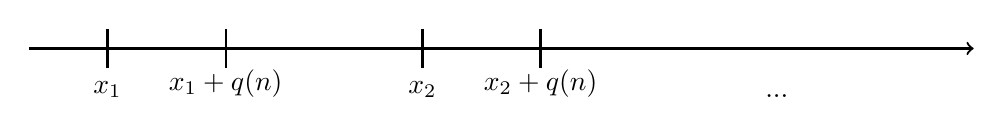
\begin{tikzpicture}
        \draw[thick, ->] (0,0)--(12,0);
        \draw[thick, -] (1, 0.25)--(1, -0.25);
        \draw (1, -0.75) node[anchor=south] {$x_1$};
        \draw[thick, -] (2.5, 0.25)--(2.5, -0.25);
        \draw (2.5, -0.75) node[anchor=south] {$x_1 + q(n)$};
        \draw[thick, -] (5, 0.25)--(5, -0.25);
        \draw (5, -0.75) node[anchor=south] {$x_2$};
        \draw[thick, -] (6.5, 0.25)--(6.5, -0.25);
        \draw (6.5, -0.75) node[anchor=south] {$x_2 + q(n)$};
        \draw (9.5, -0.75) node[anchor=south] {...};
    \end{tikzpicture}
\end{center}

Then the probability of breaking this cipher is
$$\frac{2q(n) - 1}{2^n} \cdot q(n)$$

In practice, we use block ciphers, which are stronger primitives.

\section{Message Authentication Codes}
Now we address the question of how we can guarantee the \textit{integrity} of a message.
To achieve this, we will construct a new primitive, called a \textit{message authentication code}, or MAC for short. MACs generate a verifiable tag $t$ for a message $m$ that cannot be forged.

When sending a message, Alice sends the pair $(m, t)$.
Once Bob receives the message, he runs $\Verify(k, m, t)$.
He accepts the message if $\Verify(k, m, t) = 1$, otherwise he rejects the message.
The formal definition is stated below:
\begin{definition}[Private-Key Encryption Scheme]
    A MAC scheme $\Pi$ is a tuple of algorithms $\Pi = (\gen, \mac, \Verify)$, with the following syntax:
    \begin{enumerate}
        \item $k \leftarrow \gen(1^n)$
        \item $t \leftarrow \mac(k,m)$
        \item $0/1 \leftarrow \Verify(k, m, t)$
    \end{enumerate}
    where $n$ is a security parameter and $k, m \in \{0, 1\}^{l(n)}$
\end{definition}

We impose the following \textit{correctness} requirement on our MACs:
\begin{definition}[MAC Correctness]
    $$\forall n, k \in \gen(1^n), m \in \{0, 1\}^*, \Pr[\Verify(k, m, \mac(k, m)) = 1] = 1$$
\end{definition}

We also want the message authentication codes to be \textit{unforgeable}.
That is, given a message $m$, a nu-PPT attacker $\ma$ should only be able to forge a tag $t$ for $m$ with negligible probability.
\begin{definition}[EUF-CMA Security]
    A MAC scheme $\Pi = (\gen,\mac,\Verify)$ is EUF-CMA-secure if $\forall$ nu-PPT $\ma$,
    $$\Big| \Pr\left[\mathsf{MAC}\pcmathhyphen{}\mathsf{forge}_{\cA, \Pi}(\secpar) =1\right]\Big| = \negl$$
\end{definition}

\begin{definition}[$\mathsf{MAC}\pcmathhyphen{}\mathsf{forge}_{\cA, \Pi}(\secpar)$]
$ $
   \begin{enumerate}
        \item \textbf{Setup:} The challenger samples $k$ uniformly from the key space. $\cA$ is given $1^n$.
        \item \textbf{Query:} The adversary submits a message $m^{(i)}$; then the challenger computes a tag $t^{(i)} \gets \mac(k, m^{(i)})$ and sends it to the adversary. The adversary may submit any polynomial number of message queries.
        
        Let $\mathcal{Q} = \{(m^{(1)}, t^{(1)}), \dots, (m^{(q)}, t^{(q)})\}$ be the set of messages $m^{(i)}$ submitted in the query phase along with the tags $t^{(i)}$ computed by $\mac$.
        \item \textbf{Forgery:} The adversary outputs a message-tag pair $(m^*, t^*)$. The output of the game is $1$ if $(m^*,t^*) \notin \mathcal{Q}$ and $\Verify(k, m^*, t^*) = 1$. The output is $0$ otherwise.
    \end{enumerate}
\end{definition}


%\marginnote[-1.5in]{
%\procedureblock[linenumbering]{$ \pcnotionstyle{OLDPri\pcmathhyphen{}}\indcpa_{\Pi}^{\adv}(\secpar)$}{
% b \sample \bin \\
%  \key  \sample \gen ( \secparam ) \\
% ( \state ,m_0 ,m_1) \sample \adv^{\enc ( \key ,\cdot )} ( \secparam) \\
% c \sample \enc ( \key ,m_b ) \\
% b' \sample \adv^{\enc ( \key ,\cdot )} ( \state , c ) \\
% \pcreturn b = b' }
% }

 